% Chapter Template

\chapter{Analysis and Results - Active Monitoring} % Main chapter title

\label{Chapter6} % Change X to a consecutive number; for referencing this chapter elsewhere, use \ref{ChapterX}

\lhead{Chapter 6. \emph{Analysis and Results -  Active Monitoring}} % Change X to a consecutive number; this is for the header on each page - perhaps a shortened title

%----------------------------------------------------------------------------------------
%	SECTION 1
%----------------------------------------------------------------------------------------

%Trying to associate -> rejected some time -> status code = 12 ?
%Connecté et puis disconection abrupte -> code = 3 ?


\section{Analysis}
This chapter focus on the analysis made by our probe. This device simulates a lambda user that tries to establish a connection to the UCL's wireless network in order to access the Internet. The procedure followed by the device is quite simple. For each \texttt{SSID} available on the campus the process is the following.

\begin{enumerate}
\item Associate with the access point
\item Get an \texttt{IP} address
\item Check the availability of a set of services
\end{enumerate}

The goal here is to get an overview of the infrastructure from the user's point of view. It is something really interesting because most of the time, the administrators make their diagnosis only by looking at the states of the components that they directly managed. Here, we try to complete those observations adding an opposite view (i.e. the view of the devices that use the infrastructure).

The purpose of the active monitoring is, as mentioned before, to simulate a user on the network and make a bunch of tests in order to get a live overview of the network status. During the connection loop, a various set of data are gathered and inserted into log files. We have decided to focus on several metrics. As a reminder, here are the information available into a typical log file.

\begin{description}
	\item[Scan results]: The set of access points around the device as well as other \texttt{RF} related information.
	\item[AP tried]: The set of access points that the device tries to associate with.
	\item[AP connected]: The set of access points that the device has associated with during the tests. Like most devices, our router may change the access point to a better one (i.e. roaming).
	\item[Supplication Time]: Time elapsed during the connection establishment.
	\item [DHCP Time]: Time elapsed till an \texttt{IP} address is assigned to the device.
	\item [Services checks]: The results of the services availability tests.
\end{description}

Those information are stored and analyzed by the server. By aggregating those gathered data throughout time, we can build an estimation of the overall quality experienced by the users.

\section{Scanning}
As detailed above, the first part of the log file aggregates all the scan results performed by the supplicant before connecting to a network. Those information are quite interesting since they allow us to get live details about the current environment of the router. Thanks to those results we have a full overview of the signal strength of all the surrounding access points as well as their frequencies and the \texttt{SSID} they broadcast. 


\paragraph*{Current Wifi Environment} On the web platform, we can see the lastest scan results sent by the device. This can help the administrator to diagnose some \emph{dead zones} on the campus. The results we have are the exact surroundings of the router itself and by consequence we can directly tell if the area where the probe is located is correctly covered or not. We could have chosen to plot the signal strength throughout the day but in our situation the \texttt{RF} environment is quite stable and we prefer to provide the most recent scan results. Nevertheless, such analysis could be interesting for administrators that desire to monitor a room where the \texttt{RF} conditions significantly vary. All the data required are already available in the database to support that extension.

\paragraph*{Source} The source of those data is \texttt{wpa\_supplicant} itself. Before any association, the supplicant scans the environment to detect all the reachable access points. Those results come with the a bunch of related information. The following figure represents a typical scan result displayed on the web interface.

\begin{figure}[H]
	\centering
   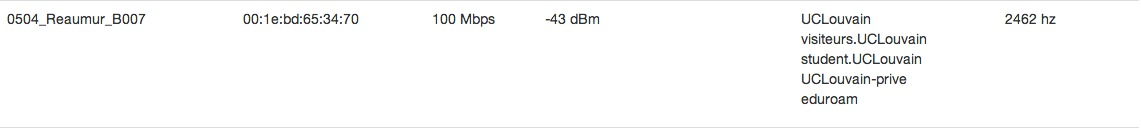
\includegraphics[width=1\textwidth]{Pictures/chapter6/scan-result.jpg}
   \caption{Example of a scan result}
\end{figure} 


\section{Access Points Interactions}
During the connection establishment phase, the supplicant makes several interactions with the access points. The first interaction it makes is in order for the supplicant to associate itself with one of the access points. The others concerns all the required data exchanges for the \texttt{802.1X} authentication process.

\subsection{Access Point Association}
The algorithm used by the supplicant is quite straightforward. It lists the access point that broadcast the \texttt{SSID}, the client wants to connect to, in a decreasing order based on the signal strength. The connection routine of \texttt{wpa\_supplicant} then tries to associate to those APs starting with the best one.

\paragraph*{Rejection} The first observation we made was that our device does not always connect with the best access point. Indeed, it may sometimes be rejected by several APs before being able to complete the association phase. This is an issue since our device might be associated to an access point with a weaker signal than other potential ones. This is a perfect example of why such active analysis can be useful. During our investigations we have noticed that each time an association is rejected, the status code is equal to \texttt{12}. By looking into the \texttt{wpa\_supplicant} source code\footnote{ieee802\_11\_defs.h} we have found that this status code refers to \texttt{WLAN\_STATUS\_ASSOC\_DENIED\_UNSPEC} that states for \emph{Access Denied Unspecified}. Our monitoring tool was able to detect the issue but a deeper debugging on the access point and the device is required in order to find the precise cause. That is outside the scope of our system since we do not have a direct access to the APs nor the controller in order to perform a deeper analysis. Nevertheless, we record all the tried access point and we are able to provide the quantity of APs that has rejected the association. With that metric, and by crossing it with the scan results, we are able to tell where that issue occurred. Here are the messages received from the \texttt{wpa\_supplicant} daemon by our application when an association reject occurs.\\

\begin{lstlisting}[frame=single,breaklines=true,caption={Exemple of rejection}]
Trying to associate with XX:XX:XX:XX:XX:XX (SSID='student.UCLouvain' freq=2437 MHz)
CTRL-EVENT-ASSOC-REJECT bssid=XX:XX:XX:XX:XX:XX status_code=12
\end{lstlisting}

\paragraph*{Deconnection} Another problem reported during our analysis was the fact that the device randomly disconnects and reconnects during the test. Even if such behavior is totally normal for a common user since it is interpreted as roaming, it is quite disturbing for our tests. Indeed, those reconnections interrupt the test and make them running on different access points. Like before, we have recorded the events generated by \texttt{wpa\_supplicant} and identified the cause. The reported error (\texttt{reason=4}) was because of an inactivity of the access point. Here again, if such issues want to be diagnosed, deeper access to the infrastructure is required. For now, we monitor the amount of reconnections during a set of tests and we are able to inform when they occur.\\

\begin{lstlisting}[frame=single,breaklines=true,caption={Example of Deconnection trace}]
CTRL-EVENT-DISCONNECTED bssid=XX:XX:XX:XX:XX:XX reason=4
Trying to associate with XX:XX:XX:XX:XX:XX (SSID='student.UCLouvain' freq=2437 MHz)
\end{lstlisting}


\paragraph*{Source} All these logs are generated by \texttt{wpa\_supplicant} and provided through an events generator mechanism. Our program is interfaced with the supplicant and is able to record all those events, parse them and insert useful information into our own log file. It offers a rich source of information in order to trace all the steps of the association.


\section{Time Durations}
Time is an important factor when dealing with wireless networks performances. Indeed, the users can be really annoyed when the connection establishment duration begins to take too much time. We have decided to keep track of the time duration it takes for \texttt{wpa\_supplicant} to establish a connection with the network. Concretely, we start a timer when the command \texttt{SELECT\_NETWORK} is sent to the control interface to start the connection phase and we stop it as soon as a \texttt{WPA-EVENT-CONNECTED} is received. We keep track of the time it takes for the \texttt{DHCP} server to provide an \texttt{IP} address to the supplicant as well. The methodology is the same as the one used for the connection establishment's duration computation. A timer is started as soon as the interface is connected to the network and before sending a \texttt{DISCOVER} message to the \texttt{DHCP} client, and is stopped as soon as a lease for an \texttt{IP} address is obtained. 

\paragraph*{Decomposition} An interesting feature of this analysis is that, as we just mentioned, we can decompose the waiting time of the user in different parts. By observing the proportion of each part, we can point out what part constitutes the bottleneck of the connection establishment. Since we gathered those indicators during our deployment phase, we are able to monitor their evolution and make the distinction between persistent problems and the isolated cases. After plotting all the data collected on a graph, we have come to conclusion that, despite the fact that are some peaks in the time duration, the connection and \texttt{DHCP} remain rather constant. Here is an example for the networks \texttt{UCLouvain-prive} and \texttt{UCLouvain} record from the \emph{Reaumur} building.

\begin{figure}[H]
	\centering
   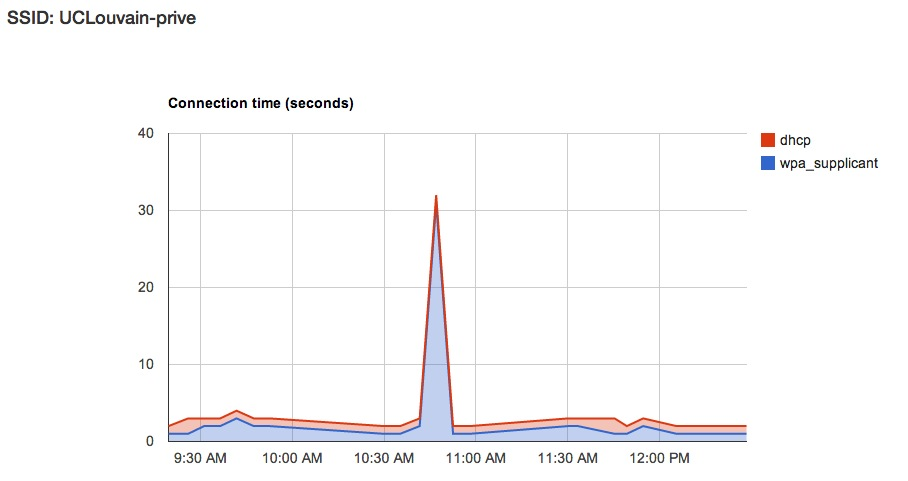
\includegraphics[width=1\textwidth]{Pictures/chapter6/time-uclouvain-prive.jpg}
   \caption{Connection time for \texttt{UCLouvain-prive}}
\end{figure} 

\begin{figure}[H]
	\centering
   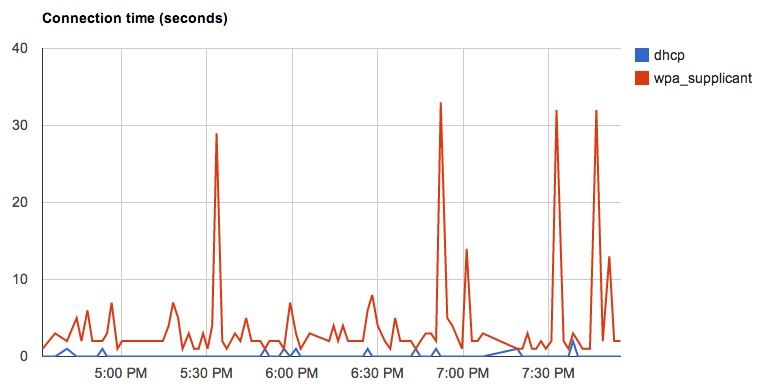
\includegraphics[width=1\textwidth]{Pictures/chapter6/time-uclouvain.jpg}
   \caption{Connection time for \texttt{UCLouvain}}
\end{figure} 

\paragraph*{Peak of time} We have investigated on the possible reasons of those peaks and we have noticed that the \texttt{wpa\_supplicant} daemon seems to spend a lot of time in the association phase. As said before, the AP is sometimes rejecting the device and, thus, forces the supplicant to associate to other ones. This may induce some latency in the connection phase and impact on perceived performance of the user. In order to understand why those rejected associations happen, we checked the log file of the \texttt{WiSM} and we found a lot of times the same \texttt{LWAPP} error message.\\
\begin{lstlisting}[frame=single,breaklines=true,caption={\texttt{WiSM} association error message}]
%LWAPP-3-INVALID_AID2: Association identifier [int] for client [hex]:[hex]:[hex]:[hex]:[hex]:[hex] is already in use by[hex]:[hex]:[hex]:[hex]:[hex]:[hex]
\end{lstlisting}

The explanation\footnote{http://www.cisco.com/c/en/us/td/docs/wireless/controller/message/guide/controller\_smg/msgs6.html} \texttt{Cisco} gives for that message is that an internal error caused an invalid association ID to be received from an AP for the indicated client and that the client may experience communications problems. This error message can also be observed for other devices on the network. In our case it might be linked to the fact that we generate a lot of associations in a short time.

\paragraph*{Source} This analysis heavily uses the event mechanism of \texttt{wpa\_supplicant} to generate its estimations of duration. We complete the analysis with the controller logs that are available on the \emph{Gathering} part. This is also a good example that a system embedding all the monitoring tools can help to generate better analysis about issues on a complex infrastructure.


\section{Services Availability}
We wanted our application to be able to give a performance and quality overview of the network every time a new connection is established. As mentioned before, we have divided our test into two parts. First we perform a \texttt{DNS} query on the two \texttt{DNS} servers of the UCL to see if both servers are reachable. Then we test the \texttt{TCP} connection to the main UCL's services added to the collection of the ten most visited website in the world with simple \texttt{socket} connections. After having received several log files from the router we were able to check the results and make some analysis on them. By decoupling those analysis, we can localize more precisely the connectivity issues.

\paragraph*{DNS} First of all, both \texttt{DNS} servers are always reachable and accessible for the five \texttt{VLANs}. The interest here comes from the fact that for the users, when the \texttt{DNS} is not responding, it the same as the \emph{Internet} is not working. 

\paragraph*{Service checks} The results of the service reachability tests depend on which network the test is executed on. Indeed, the UCL's online wireless documentation states that some \texttt{VLANs} restrict the range of accessible websites. We were able to confirm that information thanks to these tests. Upon our analysis we can see that, only two networks have some restrictions.

\begin{itemize}
	\item [-] \texttt{visiteurs.UCLouvain}
	\item [-] \texttt{UCLouvain-prive}
\end{itemize}

For the first one, all the services are reachable except \texttt{horaire.sgsi.ucl.ac.be}. This is because the port used to access this website is the port \texttt{8080} and this port has been blocked for this \texttt{VLAN}. Concerning the \texttt{UCLouvain-prive}, all the websites but the ones managed by the UCL are blocked. The exhaustive list of all the services checked is described in section \texttt{4.2.3.2}.

By checking periodically those services, we can generate their rate of availability which can be a good indicator to determine the network's performance perceived by the user.


\paragraph*{Source} The data used in this analysis are completely generated by our system. The tests are performed by subroutines implemented in our \texttt{C} program. All the information are centralized in the server that also handles all the data analysis phase.

\section{Limitations}


The main limitation of those analysis is the interface of \texttt{wpa\_supplicant}. We interface our program with it and use its message and functions to generate our data. A more powerful approach would be to work directly in the \texttt{wpa\_supplicant} code and extend it with our program. That is far more complex and would require a lot more of time. Nevertheless, it is really an interesting idea for future extensions for our system.

\section{Summary}
In this chapter, information about the analysis performed by our active monitoring program has been developed. Thanks to all the collected data plotted into graphs we were able to spot some issues on the network that we tried to understand and describe. The active tool is still a prototype but, as we have seen throughout this chapter, it can help diagnose the network with a different view since the information it is able to gather is not always reported in the controller log files.
